% Kopfzeile beim Kapitelanfang:
\fancypagestyle{plain}{
%Kopfzeile links bzw. innen
\fancyhead[L]{\Large Vorlesung 12 (21.11.2013)}
%Kopfzeile rechts bzw. außen
\fancyhead[R]{}}
%Kopfzeile links bzw. innen
\fancyhead[L]{\Large Vorlesung 12 (21.11.2013)}
%Kopfzeile rechts bzw. außen
\fancyhead[R]{}
% **************************************************
\section{Cauchy-Kriterium für Reihen}\label{7.3}
$\sum_{k=1}^\infty a_k$ konvergiert $\Lra$ die Partialsummenfolge $(s_n = \sum_{k=1}^n a_k)_{n \in \N}$ ist Cauchyfolge\\
$\Lra \forall \eps > 0 \exists n_0 \in \N: \underbrace{|s_n-s_m|}_{=|\sum_{k=1}^n a_k|} < \eps \forall n>m \ge n_0$\\
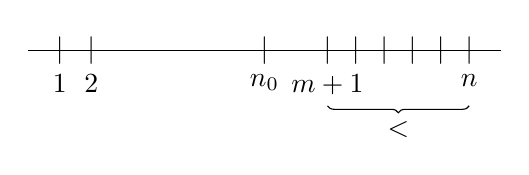
\begin{tikzpicture}
\draw(0,0)--(6,0);
\foreach \x/\xtext in {0.4/$1$,0.8/$2$,3/$n_0$,3.8/$m+1$,5.6/$n$}
  \draw(\x,0pt) node{$|$} (\x,-5pt) node[below] {\xtext};
\foreach \x in {4.16,4.52,4.88,5.24}
  \draw(\x,0pt) node{$|$};
\draw [decoration={brace,mirror,raise=0.5cm},decorate] (3.8,-0.2)--(5.6,-0.2);
\draw (4.7,-1) node{$< \eps$};
\end{tikzpicture}

\section{Korollar}\label{7.4}
Sei $\sum a_k$ konvergent $\Ra \lim_{n \to \infty} a_k = 0$

\subsection*{Beweis}
Cauchykriterium mit $n=n+1$

\subsection*{Achtung}
\enk{
\item $\lim_{k \to \infty} a_k = 0 \nRightarrow \sum_{k=1}^\infty a_k$ konvergent!\\
Beispiel: $\sum_{k=1}^\infty \frac{1}{k}$ divergiert (später), obwohl $\bigbrackets{\frac{1}{k}}$ Nullfolge
\item Ändert man endlich viele Glieder einer Reihe (oder lässt sie weg), so ändert dies das Konvergenzverhalten nicht. Der Reihenwert ändert sich aber im Allgemeinen schon!
}

\section{Regeln für konvergente Reihen}\label{7.5}
$\sum_{k=1}^\infty a_k, \sum_{k=1}^\infty b_k$ seien konvergent, $\Ra$
\en{
\item $\sum_{k=1}^\infty (a_k+b_k)$ konvergiert, $\sum_{k=1}^\infty (a_k+b_k)=\sum_{k=1}^\infty a_k + \sum_{k=1}^\infty b_k$
\item $\lambda \in \C \Ra \sum_{k=1}^\infty i(\lambda a_k)$ konvergiert gegen $\lambda \cdot \sum_{k=1}^\infty a_k$\\
Produkte von Reihen: schwieriger $\rightarrow$ später\\
Warnung: $(\sum a_k) \cdot (\sum b_k) \neq \sum a_k b_k$
}

\subsection*{Beweis}
\en{
\item $s_n = \sum_{k=1}^\infty a_k, t_n = \sum_{k=1}^n b_k, s_n \to s = \sum_{k=1}^\infty a_k, t_n \to t = \sum_{k=1}^\infty b_k$\\
$\Ra \sum_{k=1}^n (a_k+b_k) = s_n + t_n \to s+t$
\item analog
} \qed

\subsection*{Warnung}
Klammern dürfen im Allgemeinen nicht weggelassen werden!\\
Beispiel: $(1-1)+(1-1)+(1-1)+\ldots=\sum_{k=1}^\infty (1-1) = 0$
$1-1+1-1+\ldots=\sum_{k=1}^\infty (-1)^k$ divergiert!

\section{Reihen mit positiven Gliedern}\label{7.6}
Sei $a_k \in \R$ mit $a_k \ge 0 \forall k \in \N$. Dann:\\
$\sum_{k=1}^\infty a_k$ konvergiert $\Lra \bigbrackets{s_n=\sum_{k=1}^n a_k}_{n \in \N}$ ist beschränkt.

\subsection*{Beweis}
$(s_n)$ ist monoton wachsend. Monotoniekriterium (\ref{5.10}) zeigt:\\
$(s_n)$ konvergiert $\Lra (s_n)$ ist beschränkt. \qed

\section{Beispiele für konvergente/divergente Reihen}\label{7.7}
\enk{
\item $\sum_{k=1}^\infty \frac{1}{k^2}$ konvergiert. Denn:\\
$s_n = \sum_{k=1}^n \frac{1}{k^2} \le 1 + \sum_{k=2}^n \frac{1}{k(k-1)} = 1 + \sum_{k=1}^{n-1} \frac{1}{k(k+1)} \le 1+1=2$\\
$\Ra (s_n)$ beschränkt $\underset{\ref{7.6}}{\Ra} \sum \frac{1}{k^2}$ konvergiert
\item Allgemein: $s \in \N, s \ge 2 \Ra \sum_{k=1}^\infty \frac{1}{k^s}$ konvergiert (Übung)
\item \underline{Harmonische Reihe}: $\sum_{k=1}^\infty \frac{1}{k}$ divergiert. Denn:\\
$s_{2^n} = \sum_{k=1}^{2^n} \frac{1}{k} = 1 + \frac{1}{2} + (\frac{1}{3} + \frac{1}{4}) + (\underbrace{\frac{1}{5} + \ldots + \frac{1}{8}}_{4 \text{ Summanden}}) + \ldots + \bigbrackets{\underbrace{\frac{1}{2^{n-1}+1}+\ldots+\frac{1}{2^n}}_{2^{n-1} \text{ Summanden}}}$\\
$> 1 + \frac{1}{2} + 2 \cdot \frac{1}{4} + 4 \cdot \frac{1}{8} + \ldots + 2^{n-1} \cdot \frac{1}{2^n} = 1+n \cdot \frac{1}{2} \to \infty (n \to \infty) \Ra (s_n)_{n \in \N}$ ist unbeschränkt
}
Als Nächstes: Alternierende Reihen, z.B.: $1-\frac{1}{2}+\frac{1}{3}-\frac{1}{20}+\frac{1}{35} \mp \ldots$ (Glieder abwechselnd positiv/negativ)

\section{Leibniz-Kriterium für alternierende Reihen}\label{7.8}
Sei $(a_k) \subseteq \R$ mit $a_k \ge 0 \forall k$ monoton fallende Nullfolge. $\Ra$\\
\enr{
\item $\sum_{k=0}^\infty (-1)^k a_k$ konvergiert
\item \underline{Fehlerabschätzung}: $s=\sum_{k=0}^\infty (-1)^k a_k \Ra |s-\underbrace{\sum_{k=0}^n (-1)^k a_k}_{=s_n}| \le a_{n+1}$
}

\subsection*{Beweis}
$s_n = a_0 - a_1 + a_2 - a_3 \pm \ldots$\\
$s_n - s_{n-2} = (-1)^n a_n + (-1)^{n-1} a_{n-1} = (-1)^n \cdot (\underbrace{a_n - a_{n-1}}_{\le 0})$\\
Also: $\begin{array}{l l l l}
n \text{ gerade} & \Ra & s_n \le s_{n-2} & \text{das heißt: } s_0 \ge s_2 \ge s_4 \ge \ldots \\
n \text{ ungerade} & \Ra & s_n \ge s_{n-2} & \text{das heißt: } s_1 \le s_3 \le s_5 \le \ldots
\end{array}$\\
$s_0 \ge s_{2n} = s_{2n-1} + a_{2n} \ge s_{2n-1} \ge s_1$\nl
$\Ra (s_2n)_{n \in \N}$ ist monoton fallend und beschränkt, $(s_{2n-1})_{n \in \N}$ ist monoton wachsend und beschränkt.\\
$\Ra A := \lim_{n \to \infty} s_{2n}, B := \lim_{n \to \infty} s_{2n-1}$ existieren in $\R$\nl
$a_{2n} = s_{2n}-s_{2n-1} \to A-B$; Andererseits: $a_{2n} \to 0$; Also: $A=B=: s$\\
$\Ra s_n \to s$ für $s \to \infty$, das heißt, (i) sei damit gezeigt.\nl
Fehlerabschätzung: $s$ liegt zwischen $s_n$ und $s_{n+1}$\\
$\Ra |s-s_n| \le |s_{n+1}-s_n| = a_{n+1}$ \qed

\begin{tikzpicture}
\draw [->,blue](5cm,0mm) arc (-5:185:4cm);
\draw (-5,0) -- (5,0);
\draw [<-,green](3cm,0mm) arc (0:180:3cm);
\draw [->,blue](3cm,0mm) arc (-5:185:2cm);
\draw [<-,green](1cm,0mm) arc (0:180:1cm);
\draw[red] (0,5)--(0,-1) node [right]{s};
\draw [->,blue](1cm,0mm) arc (-5:185:0.75cm);
\node(0) at (5,0)[below] {$s_0=a_0$};
\node(0) at (-3,0)[below] {$s_1$};
\node(1) at (3,0)[below] {$s_2$};
\node(2) at (-1,0)[below] {$s_3$};
\node(0) at (-0.5,0)[below] {$s_5$};
\node(0) at (1,0)[below] {$s_4$};
\end{tikzpicture}\\
\emph{Vielen Dank an Helen Meyer für diese Grafik. :)}

\section{Beispiele}\label{7.9}
\enk{
\item \underline{Alternierende harmonische Reihe}:\\
$1-\frac{1}{2}+\frac{1}{3}-\frac{1}{4} \pm \ldots = \sum_{k=1}^\infty \frac{(-1)^{k-1}}{k}$ konvergiert nach Leibniz-Kriterium.\\
Sei $s$ der Reihenwert $\Ra \left|s-\sum_{k=1}^n \frac{(-1)^{k-1}}{k}\right| \le \frac{1}{n+1}$. Bem.: $s = ln 2$
\item \underline{Leibniz-Reihe}:\\
$1-\frac{1}{3}+\frac{1}{5}-\frac{1}{7} \pm \ldots = \sum_{k=0}^\infty \frac{(-1)^k}{2k+1}$ konvergiert nach Leibniz-Kriterium (gegen $\frac{\pi}{4}$).
}

\section{Definition: Absolute Konvergenz}\label{7.10}
Eine Reihe $\sum_{k=1}^\infty a_k$ ($a_k \in \C$) heißt \underline{absolut konvergent}, falls $\sum_{k=1}^\infty |a_k|$ konvergiert.

\subsection*{Beispiele}
\enk{
\item $z \in \C, |z| < 1 \Ra \sum_{n=0}^\infty z^n$ ist absolut konvergen
t. $\bigbrackets{\sum_{n=0}^\infty |z^n| = \sum_{n=0}^\infty |z|^n = \frac{1}{1-|z|}}$
\item $\sum_{k=1}^\infty \frac{(-1)^{k-1}}{k}$ ist zwar konvergent, aber nicht absolut.
}

\section{Definition: Majorantenkriterium}\label{7.11}
Sei $\sum_{k=1}^\infty a_k$ eine Reihe mit $a_k \in \C$ mit $|a_k| \le b_k \in \R \forall k \in \N$, wobei $\sum_{k=1}^\infty b_k$ konvergiere (``\underline{Konvergente Majorante}'').\\
$\Ra \sum_{k=1}^\infty a_k$ ist konvergent und auch absolut konvergent, und $\left|\sum_{k=1}^\infty a_k\right| \le \sum_{k=1}^\infty |a_k| \le \sum_{k=1}^\infty b_k$

\subsection*{Beweis}
$\sum b_k$ erfüllt das Cauchy-Kriterium $\Ra \forall \eps > 0 \exists n_0 \in \N: \forall n > m \ge n_0: \eps \ge \sum_{k=m}^n |a_k| \underset{\text{Dreiecksungl.}}{\ge} \left|\sum_{k=m}^n a_k\right| \Ra \sum a_k$ erfüllt Cauchy-Kriterium $\Ra \sum a_k$ konvergiert.\\
Ebenso $\sum |a_k|$. Ferner:\\
$\left|\sum_{k=1}^\infty a_k\right| = \left|\lim_{n \to \infty} \sum_{k=1}^n a_k\right| = \lim_{n \to \infty} \left|\sum_{k=1}^n a_k\right| \le \underbrace{\lim_{n \to \infty} \sum_{k=1}^n |a_k|}_{\sum_{k=1}^\infty |a_k|}$ \qed

\section{Korollar}\label{7.12}
Jede absolut konvergente Reihe $\sum a_k$ ist konvergent.

\subsection*{Beweis}
Majorantenkriterium mit $b_k = |a_k|$. \qed

\subsection*{Beispiel}
$\sum_{k=1}^\infty \frac{i^k}{k^3}$ konvergiert absolut, denn $\left|\frac{i^k}{k^3}\right| = \frac{1}{k^3} \le \frac{1}{k^2}$, und $\sum \frac{1}{k^2}$ ist konvergente Majorante.

\newpage

\section{Definition: Quotientenkriterium}\label{7.13}
Sei $\sum_{n=1}^\infty a_n$ eine Reihe, $a_n \in \C$.
\en{
\item Es gebe $q \in \R$ mit $0 < q < 1$ und $n_0 \in \N$ so, dass $\forall n \ge n_0: a_n \neq 0$ und $\left|\frac{a_{n+1}}{a_n}\right| \le q$\\
$\Ra \sum_{n=1}^\infty a_n$ absolut konvergent.
\item Es gebe $n_0 \in \N$ so, dass $\forall n \ge n_0: a_n \neq 0$ und $\left|\frac{a_{n+1}}{a_n}\right| \ge 1$\\
$\Ra \sum_{n=1}^\infty a_n$ divergiert. 
}

\subsection*{Beweis}
\en{
\item $n \ge n_0: |a_n| = \left|\frac{a_n}{a_{n-1}}\right| \cdot \left|\frac{a_{n-1}}{a_{n-2}}\right| \cdot \ldots \cdot \left|\frac{a_{n_0+1}}{a_{n_0}}\right| \cdot |a_{n_0}|$\\
$\le q^{n-n_0} \cdot |a_{n_0}| = c \cdot q^n, c > 0$ (unabh. von $n$)\\
$c \cdot \sum_{n=1}^\infty q^n$ ist konvergente Majorante (geometrische Reihe).
\item $n \ge n_0 \Ra |a_n| \ge |a_{n_0}| \neq 0 \Ra (a_n)$ keine Nullfolge.
} \qed